\subsection{Esercizio 15}
Eseguendo il codice \nameref{cod:15} si ottengono i seguenti risultati:

    
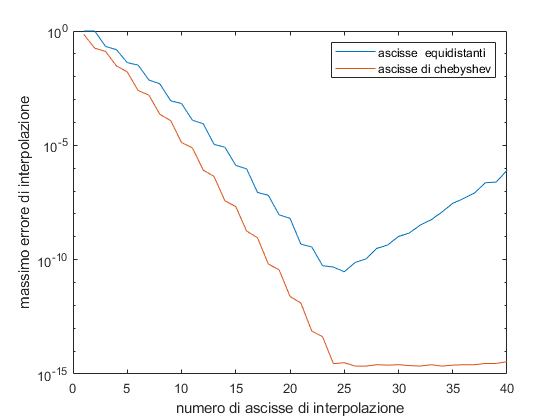
\includegraphics[scale=0.8]{capitolo4/interpol.png}

Per le ascisse di chebyshev, si ha una decrescita esponenziale dell'errore massimo per $ n \le 25$ per poi assestarsi a circa $2\cdot10^{-15}$ per n successivi.
Per quanto riguarda le ascisse equidistanti invece, si può notare come l'errore massimo torni  a crescere esponenzialmente per $n >25$. I risultati confermano
il mal condizionamento del problema di interpolazione polinomiale quando vengono usate ascisse d'interpolazione equidistanti,